\documentclass[11pt,a4paper]{article}

\usepackage[margin=2.1cm]{geometry}
\usepackage{amsmath,amssymb,amsthm,mathtools}
\usepackage{booktabs}
\usepackage{array}
\usepackage{graphicx}
\usepackage{tikz}
\usetikzlibrary{positioning,calc,arrows.meta,shapes.symbols,shapes.geometric,
  fit,backgrounds,decorations.pathmorphing}
\usepackage{enumitem}
\usepackage{longtable}
\usepackage{hyperref}
\hypersetup{colorlinks=true,linkcolor=blue!55!black,urlcolor=blue!55!black}

%%%%%%%%%%%%%%%%%%%%%%%%%%%%%%%%%%%%%%%%%%%%%%%%%%%%%%%%%%%%%%%%%%%%%%%%%%%%%%%
%  Diagram styles
%%%%%%%%%%%%%%%%%%%%%%%%%%%%%%%%%%%%%%%%%%%%%%%%%%%%%%%%%%%%%%%%%%%%%%%%%%%%%%%
\tikzset{
  wire/.style    = {line width=0.6pt},
  iwire/.style   = {line width=0.6pt, densely dashed},
  bdot/.style    = {circle, draw, fill=black, inner sep=0pt, minimum size=4.2pt},
  wdot/.style    = {circle, draw, fill=white, inner sep=0pt, minimum size=4.8pt},
  fbox/.style    = {draw, fill=white, rounded corners=1.2pt, minimum width=9mm,
                    minimum height=9mm, inner sep=2pt, font=\small},
  gbox/.style    = {draw, fill=white, signal, signal to=east,
                    signal pointer angle=120, minimum width=9mm,
                    minimum height=6.5mm, inner sep=2pt, font=\small},
  scap/.style    = {draw, fill=black!8, circle, inner sep=0.6pt, font=\scriptsize},
  bnd/.style     = {draw, fill=black!4, rounded corners=1pt, inner sep=2pt,
                    font=\scriptsize},
  lbl/.style     = {font=\scriptsize, inner sep=1.5pt},
  lblb/.style    = {font=\scriptsize, inner sep=1.5pt, text=black!65},
}

\newcommand{\dg}[1]{%
  \begin{tikzpicture}[baseline=(bl.base)]%
    \path (0,-0.6ex) node[inner sep=0,outer sep=0] (bl) {};#1%
  \end{tikzpicture}}

% ---- inline alphabet -------------------------------------------------------
% a family: box with one index leg on the left, value wire on the right
\newcommand{\dFam}[1]{\dg{\node[fbox](f){#1};%
  \draw[iwire](f.west)--++(-0.85,0);\draw[wire](f.east)--++(0.8,0);}}
% supremum cap closing an index leg
\newcommand{\dCap}{\dg{\node[scap](s){$\bigsqcup$};\draw[iwire](s.east)--++(0.8,0);}}
\newcommand{\dCapI}{\dg{\node[scap](s){$\bigsqcap$};\draw[iwire](s.east)--++(0.8,0);}}
% one-index family with its index summed away
\newcommand{\dSup}[1]{\dg{\node[fbox](f){#1};%
  \node[scap,left=6mm of f](s){$\bigsqcup$};\draw[iwire](s)--(f);%
  \draw[wire](f.east)--++(0.8,0);}}
\newcommand{\dInf}[1]{\dg{\node[fbox](f){#1};%
  \node[scap,left=6mm of f](s){$\bigsqcap$};\draw[iwire](s)--(f);%
  \draw[wire](f.east)--++(0.8,0);}}
\newcommand{\dCopy}{\dg{\node[bdot](c){};\draw[iwire](-0.8,0)--(c);%
  \draw[iwire](c)..controls(0.35,0)and(0.4,0.3)..(0.9,0.3);%
  \draw[iwire](c)..controls(0.35,0)and(0.4,-0.3)..(0.9,-0.3);}}
\newcommand{\dAdd}{\dg{\node[wdot](a){};%
  \draw[wire](-0.9,0.3)..controls(-0.4,0.3)and(-0.35,0)..(a);%
  \draw[wire](-0.9,-0.3)..controls(-0.4,-0.3)and(-0.35,0)..(a);%
  \draw[wire](a)--(0.75,0);}}

\providecommand{\bigsqcap}{}
\renewcommand{\bigsqcap}{\mathop{\rotatebox[origin=c]{180}{$\bigsqcup$}}}
\newcommand{\lean}[1]{\texttt{\small #1}}
\newcommand{\Rzi}{\mathbb{R}_{\geq 0}^{\infty}}
\newcommand{\Ninf}{\mathbb{N}^{\infty}}
\newcommand{\Card}{\mathrm{Card}}

\emergencystretch=3em
\sloppy

\theoremstyle{definition}
\newtheorem{definition}{Definition}[section]
\theoremstyle{plain}
\newtheorem{proposition}[definition]{Proposition}
\newtheorem{lemma}[definition]{Lemma}
\newtheorem{theorem}[definition]{Theorem}
\newtheorem{corollary}[definition]{Corollary}
\theoremstyle{remark}
\newtheorem{remark}[definition]{Remark}
\newtheorem{pattern}{Pattern}

\title{\bf Merging Two Index Wires\\[2mm]
\large Graphical linear algebra for the diagonal laws of suprema\\
\large on $\Rzi$, $\Ninf$ and $\Card$}
\author{Drawn proofs, machine-checked in Lean~4}
\date{}

\begin{document}
\maketitle
\vspace{-6mm}

\begin{abstract}
\noindent
A complete lattice is already a graphical linear algebra: the join $\bigsqcup$
is an infinitary white \emph{addition spider}, and on $\Rzi$, $\Ninf$ or
$\Card$ the second operation $+$ is a box that slides through that spider.
In this calculus a family $f\colon\iota\to\alpha$ is a box with one
\emph{index leg}, and taking a supremum is \emph{closing} that leg with a cap.
The lemmas of this note are then all one picture: a diagram with two index legs
closed independently equals the same diagram with the two legs joined by a
\emph{copy node} and closed once --- provided the diagonal is cofinal.
We draw the law, its reflection for infima, its bounded (conditionally
complete) form, its rig form
$(\bigsqcup f)+(\bigsqcup g)=\bigsqcup_k\,(f_k+g_k)$, and its instances on
$\Rzi$, $\Ninf$ and $\Card$; we also draw the counterexample that shows the
side condition cannot be dropped. Every named claim is machine-checked in the
Lean~4 file \lean{RequestProject/LatticeDiagrams.lean}.
\end{abstract}

\tableofcontents

%%%%%%%%%%%%%%%%%%%%%%%%%%%%%%%%%%%%%%%%%%%%%%%%%%%%%%%%%%%%%%%%%%%%%%%%%%%%%%%
\section{The calculus: index wires, boxes, caps}
%%%%%%%%%%%%%%%%%%%%%%%%%%%%%%%%%%%%%%%%%%%%%%%%%%%%%%%%%%%%%%%%%%%%%%%%%%%%%%%

\begin{center}
\fbox{\begin{minipage}{0.95\textwidth}
\textbf{Conventions.} Diagrams are read \textbf{left to right}. A
\textbf{dashed wire} carries an \emph{index} (an element of the index sort
$\iota$); a \textbf{solid wire} carries a \emph{value} (an element of the
lattice $\alpha$). A box \dFam{$f$} is a family: feed it an index, it
produces a value. The grey cap \dCap \emph{closes} an index leg by taking
the supremum over it, so \dSup{$f$} is $\bigsqcup_i f_i$; the dual cap
\dCapI\ takes the infimum. The black node \dCopy\ copies an index --- it is
the \emph{diagonal}. The white node \dAdd\ is the value-level addition
of $\Rzi$, $\Ninf$ or $\Card$.
\end{minipage}}
\end{center}

\medskip

The notation is the tensor-network one: a \emph{free} index leg is a dangling
wire and a \emph{contracted} index is a closed one, except that the
contraction is a supremum instead of a sum. That is not an analogy. In a
complete lattice, $(\bigsqcup,\bot)$ is a commutative, idempotent, infinitary
monoid, which is exactly the white spider of graphical linear algebra; and on
each of $\Rzi$, $\Ninf$, $\Card$ the operation $+$ distributes over
$\bigsqcup$ in each argument, which is exactly the statement that the
$+$-box slides along a wire through the spider. So $(\alpha,\bigsqcup,+)$ is a
rig and the usual diagrammatic reasoning applies verbatim.

\medskip
\begin{center}
\renewcommand{\arraystretch}{1.45}
\begin{tabular}{@{}lll@{}}
\toprule
\textbf{Picture} & \textbf{Order theory} & \textbf{Lean}\\
\midrule
dashed wire & an index variable $i:\iota$ & \lean{i : $\iota$}\\
solid wire & a lattice value & \lean{a : $\alpha$}\\
box with one index leg & a family $f:\iota\to\alpha$ & \lean{f : $\iota$ → $\alpha$}\\
box with two index legs & a doubly indexed family & \lean{f : $\iota$ → $\iota$ → $\alpha$}\\
cap $\bigsqcup$ on a leg & supremum over that index & \lean{⨆ i, f i}\\
cap $\bigsqcap$ on a leg & infimum over that index & \lean{⨅ i, f i}\\
copy node on an index & the diagonal $k\mapsto f\,k\,k$ & \lean{fun k => f k k}\\
white $+$ node & addition of values & \lean{a + b}\\
a cap with no legs left & the empty join $\bot$ & \lean{⊥} \;(=\;\lean{0} on $\Rzi$)\\
\bottomrule
\end{tabular}
\end{center}

\subsection{The four structural rules}

Everything below is derived from these, each of which is a one-line fact about
complete lattices.

\medskip
\noindent\textbf{(R1) Spider fusion.} Two caps in a row may be closed in either
order, and a cap on a $\bigsqcup$ is a single cap over the pair of indices:
\[
\bigsqcup_i \bigsqcup_j f\,i\,j \;=\; \bigsqcup_j \bigsqcup_i f\,i\,j
\;=\;\bigsqcup_{(i,j)} f\,i\,j .
\]

\medskip
\noindent\textbf{(R2) Monotonicity.} A box may be replaced by a pointwise
larger box under a cap: if $f\,i\le g\,i$ for all $i$ then
$\bigsqcup f\le\bigsqcup g$. Diagrammatically, $\le$ propagates rightwards
through every diagram.

\medskip
\noindent\textbf{(R3) Plugging.} A cap dominates each of its instances:
$f\,k\le\bigsqcup_i f\,i$ for every $k$. Drawn: replacing a cap by a chosen
input can only decrease the value.

\medskip
\noindent\textbf{(R4) Sliding.} The $+$-box slides through a cap:
\[
\Bigl(\bigsqcup_i f\,i\Bigr)+b=\bigsqcup_i\,(f\,i+b),
\qquad
a+\bigsqcup_j g\,j=\bigsqcup_j\,(a+g\,j)
\qquad(\iota\ \text{inhabited}).
\]
This is where $\Rzi$, $\Ninf$ and $\Card$ are used; a bare complete lattice has
no such box. The inhabitedness proviso is genuine: with $\iota$ empty the left
side is $\bot+b=b$ and the right side is $\bot$.

%%%%%%%%%%%%%%%%%%%%%%%%%%%%%%%%%%%%%%%%%%%%%%%%%%%%%%%%%%%%%%%%%%%%%%%%%%%%%%%
\section{The side condition, drawn}
%%%%%%%%%%%%%%%%%%%%%%%%%%%%%%%%%%%%%%%%%%%%%%%%%%%%%%%%%%%%%%%%%%%%%%%%%%%%%%%

\begin{definition}[\lean{GLA.DiagCofinal}]
A doubly indexed family $f$ is \emph{diagonally cofinal} when every entry is
dominated by a diagonal entry:
$\forall i\,j,\ \exists k,\ f\,i\,j\le f\,k\,k$.
The reflected condition, \lean{GLA.DiagCoinitial}, asks
$\forall i\,j,\ \exists k,\ f\,k\,k\le f\,i\,j$.
\end{definition}

The picture of the condition is: \emph{any two separate index inputs may be
merged into one copied input, at the cost of moving to a possibly different
index}.

\begin{center}
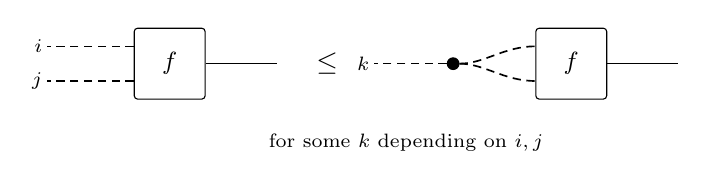
\begin{tikzpicture}
  % LHS: two free legs
  \node[fbox] (f) at (0,0) {$f$};
  \draw[iwire] (f.west)++(0,0.22)--++(-1.1,0) node[lbl,left]{$i$};
  \draw[iwire] (f.west)++(0,-0.22)--++(-1.1,0) node[lbl,left]{$j$};
  \draw[wire] (f.east)--++(0.9,0);
  \node at (2.0,0) {$\le$};
  % RHS: copy node
  \node[fbox] (g) at (5.1,0) {$f$};
  \node[bdot] (c) at (3.6,0) {};
  \draw[iwire] (c)..controls+(0.4,0)and+(-0.4,0)..($(g.west)+(0,0.22)$);
  \draw[iwire] (c)..controls+(0.4,0)and+(-0.4,0)..($(g.west)+(0,-0.22)$);
  \draw[iwire] (c)--++(-1.0,0) node[lbl,left]{$k$};
  \draw[wire] (g.east)--++(0.9,0);
  \node[lbl] at (3.0,-1.0) {for some $k$ depending on $i,j$};
\end{tikzpicture}
\end{center}

\noindent
Read the black node as ``one index, used twice''. Diagonal cofinality says the
copied form is \emph{cofinal} among the uncopied ones: nothing is lost by
insisting that the two legs carry the same index, as long as we are allowed to
choose which index.

\begin{pattern}[when the side condition is free]
If $\iota$ is a directed preorder, $f$ and $g$ are monotone families and
$\mathrm{op}$ is monotone in both arguments, then
$(i,j)\mapsto \mathrm{op}\,(f\,i)\,(g\,j)$ is diagonally cofinal: take $k$
above both $i$ and $j$. This is \lean{GLA.diagCofinal\_of\_monotone}, and it
is how the condition is met in practice (monotone sequences indexed by
$\mathbb{N}$, or by a directed family of finite subsets).
\end{pattern}

%%%%%%%%%%%%%%%%%%%%%%%%%%%%%%%%%%%%%%%%%%%%%%%%%%%%%%%%%%%%%%%%%%%%%%%%%%%%%%%
\section{The merge law}
%%%%%%%%%%%%%%%%%%%%%%%%%%%%%%%%%%%%%%%%%%%%%%%%%%%%%%%%%%%%%%%%%%%%%%%%%%%%%%%

\begin{theorem}[\lean{GLA.iSup\textsubscript{2}\_eq\_iSup\_diag}]\label{thm:merge}
Let $\alpha$ be a complete lattice and $f:\iota\to\iota\to\alpha$ diagonally
cofinal. Then
\[
\bigsqcup_i\ \bigsqcup_j\ f\,i\,j \;=\; \bigsqcup_k\ f\,k\,k .
\]
\end{theorem}

\noindent In pictures:

\begin{center}
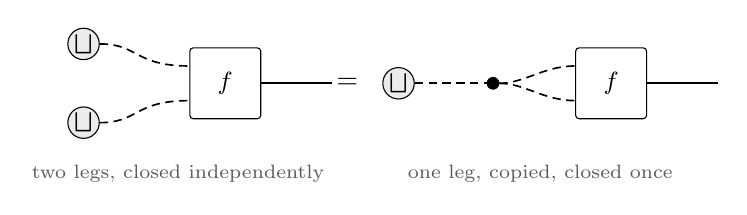
\begin{tikzpicture}
  % LHS
  \node[fbox] (f) at (0,0) {$f$};
  \node[scap] (s1) at (-1.8,0.5) {$\bigsqcup$};
  \node[scap] (s2) at (-1.8,-0.5) {$\bigsqcup$};
  \draw[iwire] (s1)..controls+(0.7,0)and+(-0.7,0)..($(f.west)+(0,0.22)$);
  \draw[iwire] (s2)..controls+(0.7,0)and+(-0.7,0)..($(f.west)+(0,-0.22)$);
  \draw[wire] (f.east)--++(0.9,0);
  \node at (1.55,0) {$=$};
  % RHS
  \node[fbox] (g) at (4.9,0) {$f$};
  \node[bdot] (c) at (3.4,0) {};
  \node[scap] (s3) at (2.2,0) {$\bigsqcup$};
  \draw[iwire] (s3)--(c);
  \draw[iwire] (c)..controls+(0.4,0)and+(-0.4,0)..($(g.west)+(0,0.22)$);
  \draw[iwire] (c)..controls+(0.4,0)and+(-0.4,0)..($(g.west)+(0,-0.22)$);
  \draw[wire] (g.east)--++(0.9,0);
  \node[lblb] at (-0.6,-1.15) {two legs, closed independently};
  \node[lblb] at (4.0,-1.15) {one leg, copied, closed once};
\end{tikzpicture}
\end{center}

\subsection*{Drawn proof}

The equality is two inequalities; each is one structural rule applied once.

\medskip
\noindent\textbf{($\ge$) The diagonal is an instance.} By (R3) applied twice,
plugging the same $k$ into both legs is one particular way of filling them, so
the doubly capped diagram dominates the diagonal one for every $k$; closing the
remaining leg by (R2) gives $\bigsqcup_k f\,k\,k \le \bigsqcup_i\bigsqcup_j f\,i\,j$.

\begin{center}
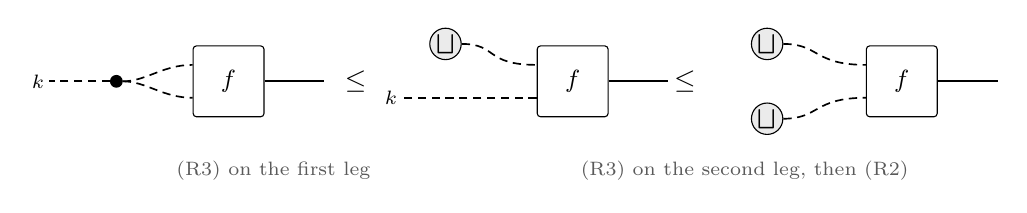
\begin{tikzpicture}[scale=0.95]
  \node[fbox] (g) at (0,0) {$f$};
  \node[bdot] (c) at (-1.5,0) {};
  \draw[iwire] (c)..controls+(0.4,0)and+(-0.4,0)..($(g.west)+(0,0.22)$);
  \draw[iwire] (c)..controls+(0.4,0)and+(-0.4,0)..($(g.west)+(0,-0.22)$);
  \draw[iwire] (c)--++(-0.9,0) node[lbl,left]{$k$};
  \draw[wire] (g.east)--++(0.8,0);
  \node at (1.7,0) {$\le$};
  \node[fbox] (h) at (4.6,0) {$f$};
  \node[scap] (t1) at (2.9,0.5) {$\bigsqcup$};
  \draw[iwire] (t1)..controls+(0.7,0)and+(-0.7,0)..($(h.west)+(0,0.22)$);
  \draw[iwire] ($(h.west)+(0,-0.22)$)--++(-1.8,0) node[lbl,left]{$k$};
  \draw[wire] (h.east)--++(0.8,0);
  \node at (6.1,0) {$\le$};
  \node[fbox] (m) at (9.0,0) {$f$};
  \node[scap] (u1) at (7.2,0.5) {$\bigsqcup$};
  \node[scap] (u2) at (7.2,-0.5) {$\bigsqcup$};
  \draw[iwire] (u1)..controls+(0.7,0)and+(-0.7,0)..($(m.west)+(0,0.22)$);
  \draw[iwire] (u2)..controls+(0.7,0)and+(-0.7,0)..($(m.west)+(0,-0.22)$);
  \draw[wire] (m.east)--++(0.8,0);
  \node[lblb] at (0.6,-1.2) {(R3) on the first leg};
  \node[lblb] at (6.9,-1.2) {(R3) on the second leg, then (R2)};
\end{tikzpicture}
\end{center}

\medskip
\noindent\textbf{($\le$) Cofinality bends the pair onto the diagonal.} Fix $i$
and $j$ and choose $k$ with $f\,i\,j\le f\,k\,k$: this is exactly the side
condition, and it replaces the two-legged diagram by a copied one. By (R3) the
copied diagram is below $\bigsqcup_k f\,k\,k$. Since $i,j$ were arbitrary, both
caps may be reinstated by (R2):

\begin{center}
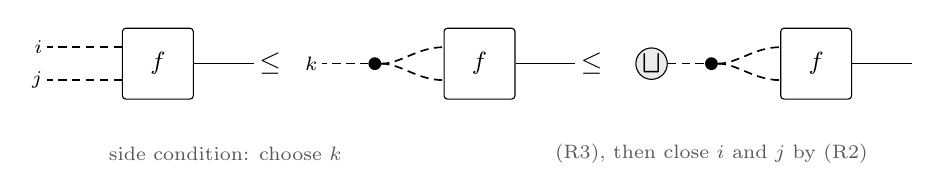
\begin{tikzpicture}[scale=0.95]
  \node[fbox] (f) at (0,0) {$f$};
  \draw[iwire] ($(f.west)+(0,0.22)$)--++(-1.0,0) node[lbl,left]{$i$};
  \draw[iwire] ($(f.west)+(0,-0.22)$)--++(-1.0,0) node[lbl,left]{$j$};
  \draw[wire] (f.east)--++(0.8,0);
  \node at (1.5,0) {$\le$};
  \node[fbox] (g) at (4.3,0) {$f$};
  \node[bdot] (c) at (2.9,0) {};
  \draw[iwire] (c)..controls+(0.35,0)and+(-0.35,0)..($(g.west)+(0,0.22)$);
  \draw[iwire] (c)..controls+(0.35,0)and+(-0.35,0)..($(g.west)+(0,-0.22)$);
  \draw[iwire] (c)--++(-0.7,0) node[lbl,left]{$k$};
  \draw[wire] (g.east)--++(0.8,0);
  \node at (5.8,0) {$\le$};
  \node[fbox] (h) at (8.8,0) {$f$};
  \node[bdot] (d) at (7.4,0) {};
  \node[scap] (s) at (6.6,0) {$\bigsqcup$};
  \draw[iwire] (s)--(d);
  \draw[iwire] (d)..controls+(0.35,0)and+(-0.35,0)..($(h.west)+(0,0.22)$);
  \draw[iwire] (d)..controls+(0.35,0)and+(-0.35,0)..($(h.west)+(0,-0.22)$);
  \draw[wire] (h.east)--++(0.8,0);
  \node[lblb] at (0.9,-1.2) {side condition: choose $k$};
  \node[lblb] at (7.4,-1.2) {(R3), then close $i$ and $j$ by (R2)};
\end{tikzpicture}
\end{center}

\noindent
That is the whole proof: \emph{merge with the side condition, plug with (R3)}.
Every later statement in this note is this picture with extra decorations.
\hfill$\square$

\subsection{Reflection: the same picture upside down}

Reflecting a diagram in a horizontal axis exchanges $\bigsqcup$ with
$\bigsqcap$ and reverses every $\le$. Applying the reflection to
Theorem~\ref{thm:merge} costs nothing --- in Lean it is literally the same
proof read in the order dual $\alpha^{\mathrm{op}}$.

\begin{theorem}[\lean{GLA.iInf\textsubscript{2}\_eq\_iInf\_diag}]
If $f$ is diagonally coinitial then
$\bigsqcap_i\bigsqcap_j f\,i\,j=\bigsqcap_k f\,k\,k$.
\end{theorem}

\begin{center}
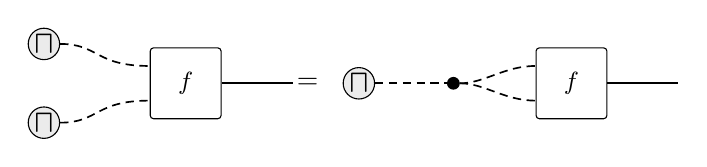
\begin{tikzpicture}
  \node[fbox] (f) at (0,0) {$f$};
  \node[scap] (s1) at (-1.8,0.5) {$\bigsqcap$};
  \node[scap] (s2) at (-1.8,-0.5) {$\bigsqcap$};
  \draw[iwire] (s1)..controls+(0.7,0)and+(-0.7,0)..($(f.west)+(0,0.22)$);
  \draw[iwire] (s2)..controls+(0.7,0)and+(-0.7,0)..($(f.west)+(0,-0.22)$);
  \draw[wire] (f.east)--++(0.9,0);
  \node at (1.55,0) {$=$};
  \node[fbox] (g) at (4.9,0) {$f$};
  \node[bdot] (c) at (3.4,0) {};
  \node[scap] (s3) at (2.2,0) {$\bigsqcap$};
  \draw[iwire] (s3)--(c);
  \draw[iwire] (c)..controls+(0.4,0)and+(-0.4,0)..($(g.west)+(0,0.22)$);
  \draw[iwire] (c)..controls+(0.4,0)and+(-0.4,0)..($(g.west)+(0,-0.22)$);
  \draw[wire] (g.east)--++(0.9,0);
\end{tikzpicture}
\end{center}

%%%%%%%%%%%%%%%%%%%%%%%%%%%%%%%%%%%%%%%%%%%%%%%%%%%%%%%%%%%%%%%%%%%%%%%%%%%%%%%
\section{Bounded diagrams: the conditionally complete case}
%%%%%%%%%%%%%%%%%%%%%%%%%%%%%%%%%%%%%%%%%%%%%%%%%%%%%%%%%%%%%%%%%%%%%%%%%%%%%%%

In a conditionally complete lattice a cap may only be attached to a
\emph{bounded} diagram. Drawing the bound as a plug $b$ that the diagram is
below:

\begin{center}
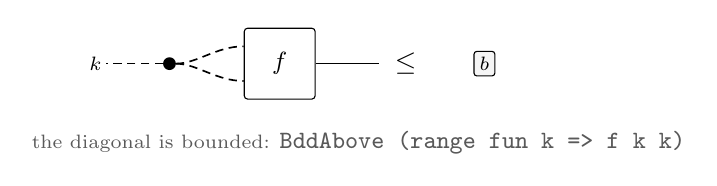
\begin{tikzpicture}
  \node[fbox] (g) at (0,0) {$f$};
  \node[bdot] (c) at (-1.4,0) {};
  \draw[iwire] (c)..controls+(0.35,0)and+(-0.35,0)..($(g.west)+(0,0.22)$);
  \draw[iwire] (c)..controls+(0.35,0)and+(-0.35,0)..($(g.west)+(0,-0.22)$);
  \draw[iwire] (c)--++(-0.8,0) node[lbl,left]{$k$};
  \draw[wire] (g.east)--++(0.8,0);
  \node at (1.6,0) {$\le$};
  \node[bnd] (b) at (2.6,0) {$b$};
  \node[lblb] at (1.0,-1.0)
    {the diagonal is bounded: \lean{BddAbove (range fun k => f k k)}};
\end{tikzpicture}
\end{center}

\noindent
The point of the section is a small but pleasant observation: \emph{the side
condition transports the bound}. If every $f\,i\,j$ sits below some diagonal
entry, and every diagonal entry sits below $b$, then the entire double family
sits below $b$ --- so all the caps in sight exist. Drawn, it is a two-step
chase:

\begin{center}
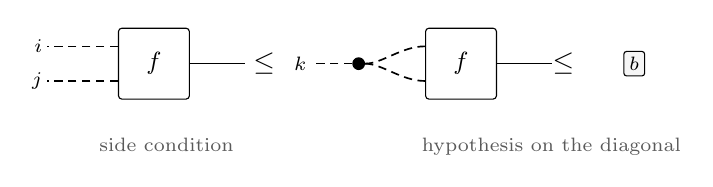
\begin{tikzpicture}
  \node[fbox] (f) at (0,0) {$f$};
  \draw[iwire] ($(f.west)+(0,0.22)$)--++(-0.9,0) node[lbl,left]{$i$};
  \draw[iwire] ($(f.west)+(0,-0.22)$)--++(-0.9,0) node[lbl,left]{$j$};
  \draw[wire] (f.east)--++(0.7,0);
  \node at (1.4,0) {$\le$};
  \node[fbox] (g) at (3.9,0) {$f$};
  \node[bdot] (c) at (2.6,0) {};
  \draw[iwire] (c)..controls+(0.3,0)and+(-0.3,0)..($(g.west)+(0,0.22)$);
  \draw[iwire] (c)..controls+(0.3,0)and+(-0.3,0)..($(g.west)+(0,-0.22)$);
  \draw[iwire] (c)--++(-0.6,0) node[lbl,left]{$k$};
  \draw[wire] (g.east)--++(0.7,0);
  \node at (5.2,0) {$\le$};
  \node[bnd] (b) at (6.1,0) {$b$};
  \node[lblb] at (3.0,-1.05)
    {side condition \hspace{2.2cm} hypothesis on the diagonal};
\end{tikzpicture}
\end{center}

\begin{theorem}[\lean{GLA.ciSup\textsubscript{2}\_eq\_ciSup\_diag}]
Let $\alpha$ be conditionally complete, $\iota$ nonempty, $f$ diagonally
cofinal, and let the diagonal $k\mapsto f\,k\,k$ be bounded above. Then
$\bigsqcup_i\bigsqcup_j f\,i\,j=\bigsqcup_k f\,k\,k$.
\end{theorem}

\begin{theorem}[\lean{GLA.ciSup\textsubscript{2}\_eq\_ciSup\_diag'}]
If moreover $\alpha$ is a conditionally complete linear order with a bottom
element, the nonemptiness hypothesis may be dropped: an empty cap is $\bot$,
and both sides of the equation collapse to $\bot$ together.
\end{theorem}

\noindent
The two proofs are the drawn proof of Theorem~\ref{thm:merge} with each use of
(R2), (R3) guarded by the bound established above: in Lean, \lean{le\_ciSup}
and \lean{ciSup\_le} in place of \lean{le\_iSup} and \lean{iSup\_le}.

%%%%%%%%%%%%%%%%%%%%%%%%%%%%%%%%%%%%%%%%%%%%%%%%%%%%%%%%%%%%%%%%%%%%%%%%%%%%%%%
\section{The rig form: two spiders with a box between them}
%%%%%%%%%%%%%%%%%%%%%%%%%%%%%%%%%%%%%%%%%%%%%%%%%%%%%%%%%%%%%%%%%%%%%%%%%%%%%%%

Now switch on the second operation. Let $\mathrm{op}$ be a value-level binary
node --- for us, always $+$ --- that slides through caps on both sides (R4).

\begin{theorem}[\lean{GLA.iSup\_op\_iSup\_diag}]\label{thm:rig}
If $\mathrm{op}$ satisfies (R4) on both arguments and
$(i,j)\mapsto\mathrm{op}\,(f\,i)\,(g\,j)$ is diagonally cofinal, then
\[
\mathrm{op}\Bigl(\bigsqcup_i f\,i\Bigr)\Bigl(\bigsqcup_j g\,j\Bigr)
= \bigsqcup_k \mathrm{op}\,(f\,k)\,(g\,k).
\]
\end{theorem}

\noindent The drawn proof is: \emph{slide, slide, merge}.

\begin{center}
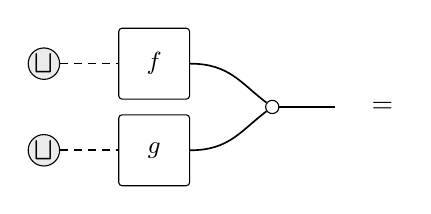
\begin{tikzpicture}
  % step 1: two capped families into a + node
  \node[fbox] (f) at (0,0.55) {$f$};
  \node[fbox] (g) at (0,-0.55) {$g$};
  \node[scap] (sf) at (-1.4,0.55) {$\bigsqcup$};
  \node[scap] (sg) at (-1.4,-0.55) {$\bigsqcup$};
  \draw[iwire] (sf)--(f); \draw[iwire] (sg)--(g);
  \node[wdot] (p) at (1.5,0) {};
  \draw[wire] (f.east)..controls+(0.5,0)and+(-0.4,0.3)..(p);
  \draw[wire] (g.east)..controls+(0.5,0)and+(-0.4,-0.3)..(p);
  \draw[wire] (p)--++(0.8,0);
  \node at (2.9,0) {$=$};
\end{tikzpicture}
\end{center}
\begin{center}
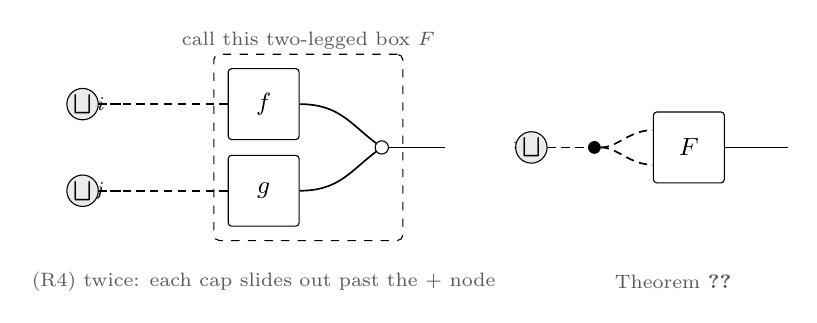
\begin{tikzpicture}
  % step 2: caps pulled out to the far left, box inside
  \node[fbox] (f) at (0,0.55) {$f$};
  \node[fbox] (g) at (0,-0.55) {$g$};
  \draw[iwire] (f.west)--++(-1.5,0) node[lbl,left]{$i$};
  \draw[iwire] (g.west)--++(-1.5,0) node[lbl,left]{$j$};
  \node[wdot] (p) at (1.5,0) {};
  \draw[wire] (f.east)..controls+(0.5,0)and+(-0.4,0.3)..(p);
  \draw[wire] (g.east)..controls+(0.5,0)and+(-0.4,-0.3)..(p);
  \draw[wire] (p)--++(0.8,0);
  \begin{scope}[on background layer]
    \node[draw,dashed,rounded corners=2pt,fit=(f)(g)(p),inner sep=5pt] (bx) {};
  \end{scope}
  \node[lblb,above] at (bx.north) {call this two-legged box $F$};
  % caps
  \node[scap] (s1) at (-2.3,0.55) {$\bigsqcup$};
  \node[scap] (s2) at (-2.3,-0.55) {$\bigsqcup$};
  \draw[iwire] (s1)--++(0.55,0); \draw[iwire] (s2)--++(0.55,0);
  \node at (3.3,0) {$=$};
  % RHS diagonal
  \node[fbox] (F) at (5.4,0) {$F$};
  \node[bdot] (c) at (4.2,0) {};
  \node[scap] (s4) at (3.4,0) {$\bigsqcup$};
  \draw[iwire] (s4)--(c);
  \draw[iwire] (c)..controls+(0.3,0)and+(-0.3,0)..($(F.west)+(0,0.22)$);
  \draw[iwire] (c)..controls+(0.3,0)and+(-0.3,0)..($(F.west)+(0,-0.22)$);
  \draw[wire] (F.east)--++(0.8,0);
  \node[lblb] at (0.0,-1.7) {(R4) twice: each cap slides out past the $+$ node};
  \node[lblb] at (5.2,-1.7) {Theorem~\ref{thm:merge}};
\end{tikzpicture}
\end{center}

\noindent
Sliding both caps out of the $+$ node turns the left-hand diagram into a
two-legged box $F\,i\,j=\mathrm{op}\,(f\,i)\,(g\,j)$ with both legs capped;
Theorem~\ref{thm:merge} then merges the legs, and merging them is precisely
running the same index through $f$ and through $g$, i.e.
$\bigsqcup_k \mathrm{op}\,(f\,k)\,(g\,k)$.

\subsection{Instances}

\begin{corollary}[\lean{GLA.ENNRealDiag.ennreal\_iSup\_add\_iSup\_diag}]
For $f,g:\iota\to\Rzi$ with $(i,j)\mapsto f\,i+g\,j$ diagonally cofinal,
\[
\bigsqcup_i f\,i \;+\; \bigsqcup_j g\,j \;=\; \bigsqcup_k\,(f\,k+g\,k).
\]
\end{corollary}

\begin{corollary}[\lean{GLA.ENNRealDiag.ennreal\_iInf\_add\_iInf\_diag}]
The reflected statement holds for infima on $\Rzi$ under the coinitial
condition:
$\bigsqcap_i f\,i+\bigsqcap_j g\,j=\bigsqcap_k\,(f\,k+g\,k)$.
\end{corollary}

\begin{corollary}[\lean{GLA.ENatDiag.enat\_iSup\_add\_iSup\_diag}]
The same statement on $\Ninf$.
\end{corollary}

\begin{corollary}[\lean{GLA.CardinalDiag.ciSup\_add\_ciSup\_diag}]
For cardinals, with $\iota$ nonempty and both $f$ and $g$ bounded above:
$\bigl(\bigsqcup_i f\,i\bigr)+\bigl(\bigsqcup_j g\,j\bigr)
=\bigsqcup_k\,(f\,k+g\,k)$ under diagonal cofinality. Here the caps are the
conditional ones, and the bound on the diagonal is manufactured from the two
given bounds by the $+$ node: if $f\,k\le b_f$ and $g\,k\le b_g$ then
$f\,k+g\,k\le b_f+b_g$.
\end{corollary}

\begin{center}
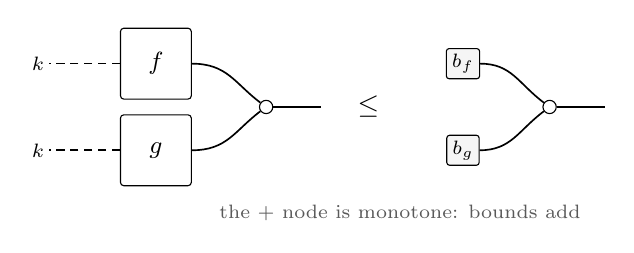
\begin{tikzpicture}
  \node[fbox] (f) at (0,0.55) {$f$};
  \node[fbox] (g) at (0,-0.55) {$g$};
  \draw[iwire] (f.west)--++(-0.9,0) node[lbl,left]{$k$};
  \draw[iwire] (g.west)--++(-0.9,0) node[lbl,left]{$k$};
  \node[wdot] (p) at (1.4,0) {};
  \draw[wire] (f.east)..controls+(0.45,0)and+(-0.4,0.3)..(p);
  \draw[wire] (g.east)..controls+(0.45,0)and+(-0.4,-0.3)..(p);
  \draw[wire] (p)--++(0.7,0);
  \node at (2.7,0) {$\le$};
  \node[bnd] (b1) at (3.9,0.55) {$b_f$};
  \node[bnd] (b2) at (3.9,-0.55) {$b_g$};
  \node[wdot] (q) at (5.0,0) {};
  \draw[wire] (b1.east)..controls+(0.4,0)and+(-0.4,0.3)..(q);
  \draw[wire] (b2.east)..controls+(0.4,0)and+(-0.4,-0.3)..(q);
  \draw[wire] (q)--++(0.7,0);
  \node[lblb] at (3.1,-1.35) {the $+$ node is monotone: bounds add};
\end{tikzpicture}
\end{center}

%%%%%%%%%%%%%%%%%%%%%%%%%%%%%%%%%%%%%%%%%%%%%%%%%%%%%%%%%%%%%%%%%%%%%%%%%%%%%%%
\section{Why the side condition cannot be dropped}
%%%%%%%%%%%%%%%%%%%%%%%%%%%%%%%%%%%%%%%%%%%%%%%%%%%%%%%%%%%%%%%%%%%%%%%%%%%%%%%

Take $\iota=\{0,1\}$ and, in $\Ninf$ (or $\Rzi$, or $\Card$),
\[
f\,0=0,\quad f\,1=1,\qquad g\,0=1,\quad g\,1=0 .
\]
Then $\bigsqcup f=\bigsqcup g=1$, so the left-hand side of the rig law is $2$,
while every diagonal entry $f\,k+g\,k$ equals $1$, so the right-hand side is
$1$. The two index wires genuinely carry different information: $f$ wants
$i=1$ and $g$ wants $j=0$, and no single $k$ satisfies both. The diagram
records this as ``the copy node is not available here''.

\begin{center}
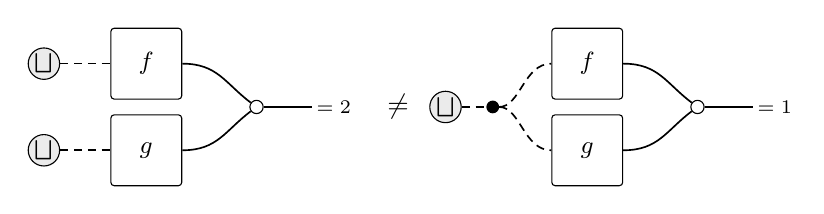
\begin{tikzpicture}
  \node[fbox] (f) at (0,0.55) {$f$};
  \node[fbox] (g) at (0,-0.55) {$g$};
  \node[scap] (sf) at (-1.3,0.55) {$\bigsqcup$};
  \node[scap] (sg) at (-1.3,-0.55) {$\bigsqcup$};
  \draw[iwire] (sf)--(f); \draw[iwire] (sg)--(g);
  \node[wdot] (p) at (1.4,0) {};
  \draw[wire] (f.east)..controls+(0.45,0)and+(-0.4,0.3)..(p);
  \draw[wire] (g.east)..controls+(0.45,0)and+(-0.4,-0.3)..(p);
  \draw[wire] (p)--++(0.7,0) node[lbl,right]{$=2$};
  \node at (3.2,0) {$\neq$};
  \node[fbox] (f2) at (5.6,0.55) {$f$};
  \node[fbox] (g2) at (5.6,-0.55) {$g$};
  \node[bdot] (c) at (4.4,0) {};
  \node[scap] (s) at (3.8,0) {$\bigsqcup$};
  \draw[iwire] (s)--(c);
  \draw[iwire] (c)..controls+(0.35,0)and+(-0.35,0)..(f2.west);
  \draw[iwire] (c)..controls+(0.35,0)and+(-0.35,0)..(g2.west);
  \node[wdot] (q) at (7.0,0) {};
  \draw[wire] (f2.east)..controls+(0.45,0)and+(-0.4,0.3)..(q);
  \draw[wire] (g2.east)..controls+(0.45,0)and+(-0.4,-0.3)..(q);
  \draw[wire] (q)--++(0.7,0) node[lbl,right]{$=1$};
\end{tikzpicture}
\end{center}

\noindent
This is checked in Lean as \lean{GLA.enat\_diag\_fails}: the two sides are $2$
and $1$ for this concrete pair of families, so the diagonal law is not a
theorem without its hypothesis.

%%%%%%%%%%%%%%%%%%%%%%%%%%%%%%%%%%%%%%%%%%%%%%%%%%%%%%%%%%%%%%%%%%%%%%%%%%%%%%%
\section{Patterns}
%%%%%%%%%%%%%%%%%%%%%%%%%%%%%%%%%%%%%%%%%%%%%%%%%%%%%%%%%%%%%%%%%%%%%%%%%%%%%%%

The proofs above reuse four moves. They are worth naming, because almost every
lemma of this shape in the order-theoretic library is one of them.

\begin{pattern}[Merge]
Two caps become one cap and a copy node when the diagonal is cofinal
(Theorem~\ref{thm:merge}). Recognise it whenever a statement has the shape
``$\bigsqcup_i\bigsqcup_j\;=\;\bigsqcup_k$ diagonal''.
\end{pattern}

\begin{pattern}[Slide]
A value-level node that distributes over $\bigsqcup$ may be pulled out of, or
pushed into, a cap. This is the only place where the specific rig
($\Rzi$, $\Ninf$, $\Card$) is used, and it is where an emptiness side condition
enters: an empty cap is $\bot$, and $\bot$ is absorbing for the slide only when
the node has $\bot$ as an annihilator on that side.
\end{pattern}

\begin{pattern}[Reflect]
Every statement about $\bigsqcup$ has a dual about $\bigsqcap$, obtained by
flipping the picture. In Lean this is instantiating the same theorem at
$\alpha^{\mathrm{op}}$, so the dual costs one line.
\end{pattern}

\begin{pattern}[Bound transport]
In a conditionally complete lattice, a cap needs a bound. Cofinality supplies
it: a bound for the diagonal is a bound for the whole double family, and a
bound for the family of row-suprema. This is what makes the conditionally
complete versions no harder than the complete ones.
\end{pattern}

\medskip
\noindent
A practical consequence, visible in the Lean file: the complete-lattice merge
law is proved once, and every other statement --- infima, conditionally
complete suprema, $\Rzi$, $\Ninf$, $\Card$ --- is obtained by \emph{reflect},
\emph{slide} and \emph{bound transport} on top of it, rather than by repeating
the $\le$/$\ge$ argument each time.

%%%%%%%%%%%%%%%%%%%%%%%%%%%%%%%%%%%%%%%%%%%%%%%%%%%%%%%%%%%%%%%%%%%%%%%%%%%%%%%
\section{Index: pictures to Lean names}
%%%%%%%%%%%%%%%%%%%%%%%%%%%%%%%%%%%%%%%%%%%%%%%%%%%%%%%%%%%%%%%%%%%%%%%%%%%%%%%

All names live in \lean{RequestProject/LatticeDiagrams.lean}, namespace
\lean{GLA}.

\begin{center}
\renewcommand{\arraystretch}{1.35}
\begin{tabular}{@{}ll@{}}
\toprule
\textbf{Statement in this note} & \textbf{Lean name}\\
\midrule
the side condition (copy node available)   & \lean{DiagCofinal}\\
its reflection                             & \lean{DiagCoinitial}\\
directed index $+$ monotone families       & \lean{diagCofinal\_of\_monotone}\\
merge law (Theorem~\ref{thm:merge})        & \lean{iSup\textsubscript{2}\_eq\_iSup\_diag}\\
reflected merge law                        & \lean{iInf\textsubscript{2}\_eq\_iInf\_diag}\\
rig form (Theorem~\ref{thm:rig})           & \lean{iSup\_op\_iSup\_diag}\\
bounded merge law                          & \lean{ciSup\textsubscript{2}\_eq\_ciSup\_diag}\\
bounded merge law, bottomed linear order   & \lean{ciSup\textsubscript{2}\_eq\_ciSup\_diag'}\\
$\Rzi$, suprema                            & \lean{ENNRealDiag.ennreal\_iSup\_add\_iSup\_diag}\\
$\Rzi$, infima                             & \lean{ENNRealDiag.ennreal\_iInf\_add\_iInf\_diag}\\
$\Ninf$, suprema                           & \lean{ENatDiag.enat\_iSup\_add\_iSup\_diag}\\
cardinals, bounded suprema                 & \lean{CardinalDiag.ciSup\_add\_ciSup\_diag}\\
the side condition is necessary            & \lean{enat\_diag\_fails}\\
\bottomrule
\end{tabular}
\end{center}

\medskip
\noindent
The file builds against Mathlib with no \lean{sorry} and no added axioms.

\end{document}
